%% LyX 2.0.3 created this file.  For more info, see http://www.lyx.org/.
%% Do not edit unless you really know what you are doing.
\documentclass[letterpaper,spanish]{article}
\usepackage[T1]{fontenc}
\usepackage[latin9]{inputenc}
\usepackage{float}
\usepackage{graphicx}

\makeatletter

%%%%%%%%%%%%%%%%%%%%%%%%%%%%%% LyX specific LaTeX commands.
\special{papersize=\the\paperwidth,\the\paperheight}


%%%%%%%%%%%%%%%%%%%%%%%%%%%%%% User specified LaTeX commands.
\date{}

\makeatother

\usepackage{babel}
\addto\shorthandsspanish{\spanishdeactivate{~<>}}

\begin{document}

\title{Informe de Parcial 3\\
Por\\
Alejandro Mesa G�mez\\
almego95@gmail.com}

\maketitle
\begin{center}
{\huge EL MOVIMIENTO PARABOLICO}\\

\par\end{center}{\huge \par}

El movimiento parab�lico es uno de los movimientos en dos dimensiones
m�s conocidos. 

El movimiento de se espec�fica indicando la rapidez inicial con la
que es lanzado un cuerpo ($\upsilon_{0}$) y el �ngulo respecto a
la superficie ($\theta$).

Si se asume que la aceleraci\'{ }n de la gravedad es $g=9.8\: m/s^{2}$
la posici�n del cuerpo en el espacio esta dada por: 

\begin{equation}
\chi=\upsilon_{0}cos\theta t
\end{equation}


\begin{equation}
y=\upsilon_{0}sin\theta t-\frac{1}{2}gt^{2}
\end{equation}


En la figura (\ref{fig:fig1}) se muestra la posici�n del cuerpo para
distintos valores de la posicion y del tiempo.

\begin{figure}[H]
\centering{}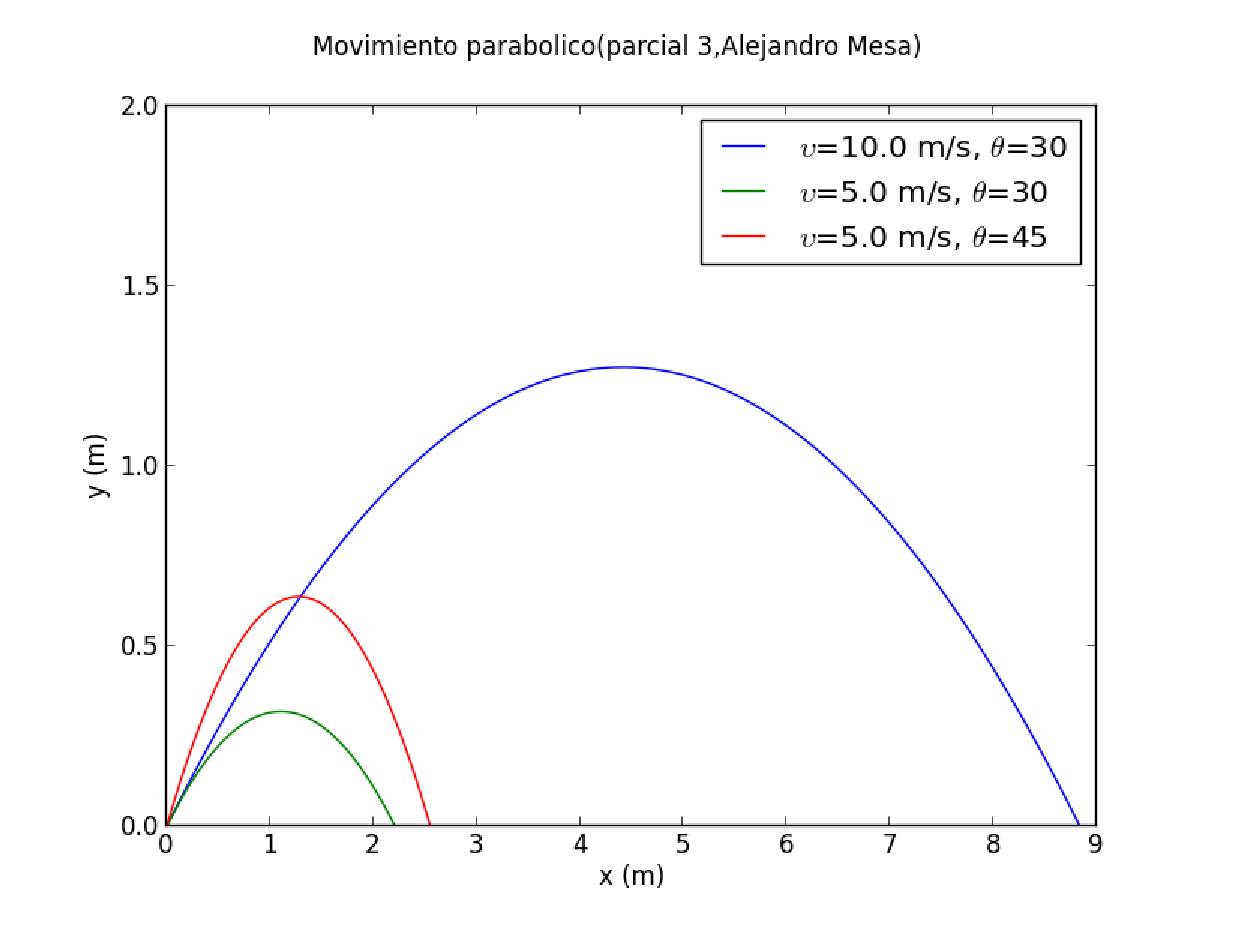
\includegraphics{figura1}\caption{Movimiento parab�lico\label{fig:fig1}}
\end{figure}

\end{document}
